%%%% EXPERIMENTAL VALIDATION %%%%
\chapter{Experimental validation of numerical simulations}\label{chap:10_Experimental_Validation}
In this chapter, we present an experimental validation of the numerical simulation framework described in \chapref{chap:06_Simulation_Framework}.
To that end, we conduct acoustical measurements corresponding to a subset of the simulations presented in \chapref{chap:08_Proposed_Method} and compare the resulting metric values between measurement and simulation.
Through these analyses, we seek to establish the domains over which our numerical simulations accurately represent reality and additionally identify any major sources of discrepancy between simulations and measurements.

\section{Experimental setup}\label{sec:10_Experimental_Validation:Experiments}
Acoustical measurements were taken in a $3.6 \times 2.35 \times 2.55$~m (length $\times$ width $\times$ height) anechoic chamber with 8-inch deep (equal to $1/4$ wavelength at $\sim425$~Hz) anechoic foam wedges.
We consider three source positions: $\vec{s}_\textrm{A} = (0.35,0,0)$~m, $\vec{s}_\textrm{B} = (0.35,0.35,0)$~m, and $\vec{s}_\textrm{C} = (0.35,0.7,0)$~m.
For each source,\footnote{Here, we use Genelec 8010A loudspeakers.} we measure, up to order $L_\textrm{in} = 4$, ambisonics impulse responses for all microphone positions $\vec{u} = (0, u_y, 0)$ with $u_y = [-0.5,0.5]$~m in increments of $0.05$~m.
(The impulse response measurement procedure is described in \apxref{chap:A5_Impulse_Response}.)
These microphone and source positions are illustrated in \figref{fig:10_Experimental_Validation:Experimental_Setup}.
The ambisonics impulse responses are then equalized by the frequency response of the same source measured by an omnidirectional reference microphone at the same position, thereby compensating for the directivity of the source.

% Diagram of source/mic positions
\begin{figure}[t]
\centering
  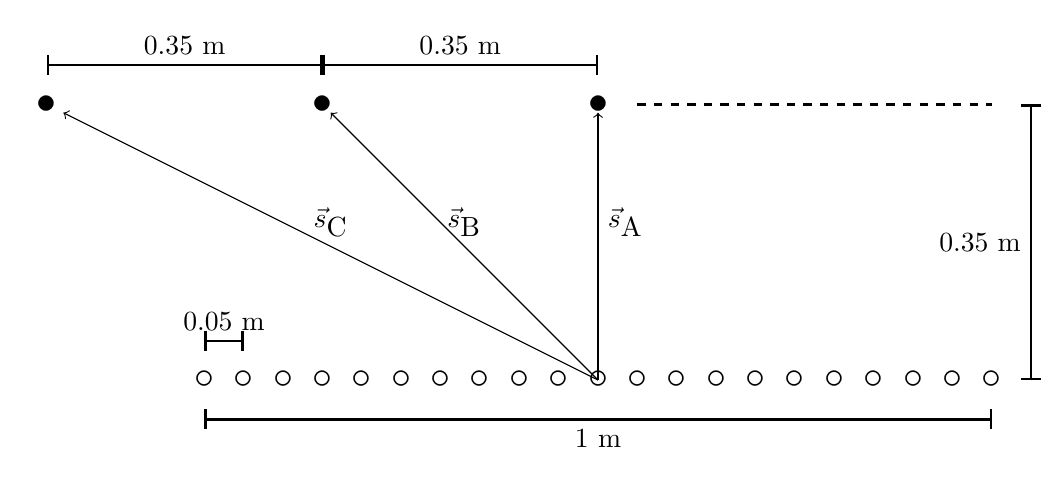
\begin{tikzpicture}[scale=10]
% Parameters
\def\radius{0.1};
\def\arrowScale{0.97};
\def\offset{0.05};

\def\micSpacing{1};
\def\micIncrement{0.05};
\def\micL{-0.5*\micSpacing};
\def\micR{0.5*\micSpacing};

\def\sourceAX{0};
\def\sourceBX{-0.35};
\def\sourceCX{-0.7};
\def\sourceY{0.35};

\pgfmathsetmacro\sourceAAzimuth{-atan(\sourceAX/\sourceY)}
\pgfmathsetmacro\sourceBAzimuth{-atan(\sourceBX/\sourceY)}
\pgfmathsetmacro\sourceCAzimuth{-atan(\sourceCX/\sourceY)}

\def\arcRadius{0.25};
\pgfmathsetmacro\arcAY{cos(-\sourceAAzimuth/2)*\arcRadius}
\pgfmathsetmacro\arcAX{sin(-\sourceAAzimuth/2)*\arcRadius}
\pgfmathsetmacro\arcBY{cos(-\sourceBAzimuth/2)*\arcRadius}
\pgfmathsetmacro\arcBX{sin(-\sourceBAzimuth/2)*\arcRadius}
\pgfmathsetmacro\arcCY{cos(-\sourceCAzimuth/2)*\arcRadius}
\pgfmathsetmacro\arcCX{sin(-\sourceCAzimuth/2)*\arcRadius}

% Coordinate system
%\draw[ultra thick,->] (0,0) -- (0,\radius);
%\draw[ultra thick,->] (0,0) -- (-\radius,0);

% Arrows
\node at (\sourceAX,\sourceY){\Large $\bullet$}; % source A
\node at (\sourceBX,\sourceY){\Large $\bullet$}; % source B
\node at (\sourceCX,\sourceY){\Large $\bullet$}; % source C
\draw[->] (0,0) -- (\arrowScale*\sourceAX,\arrowScale*\sourceY) node[above right, pos=0.5]{$\vec{s}_\textrm{A}$}; % source A
\draw[->] (0,0) -- (\arrowScale*\sourceBX,\arrowScale*\sourceY) node[above, pos=0.5]{$\vec{s}_\textrm{B}$}; % source B
\draw[->] (0,0) -- (\arrowScale*\sourceCX,\arrowScale*\sourceY) node[above, pos=0.5]{$\vec{s}_\textrm{C}$}; % source C

% Arcs
%\draw[domain=90:(90+\sourceBAzimuth)] plot ({\arcRadius*cos(\x)}, {\arcRadius*sin(\x)});
%\node at (1.15*\arcBX,1.15*\arcBY){$\varphi_\textrm{B}$};

% Mic positions
\foreach \i in {0,...,20}
{
\node at (\micL + \i*\micIncrement,0){\Large $\circ$};
}
%\node at (0,0){\Large $\circ$};
%\node at (\micL,0){\Large $\circ$};
%\node at (\micR,0){\Large $\circ$};

% Length measurements
\draw[thick,|-|] (\micL,-\offset) -- (\micR,-\offset) node[below, pos=0.5]{$1$~m};
\draw[thick,|-|] (\micL,\offset) -- (\micL+\micIncrement,\offset) node[above, pos=0.5]{$0.05$~m};
\draw[thick,|-|] (\micR+\offset,0) -- (\micR+\offset,\sourceY) node[left, pos=0.5]{$0.35$~m};
\draw[thick,dashed,-] (\micIncrement,\sourceY) -- (\micR,\sourceY);
\draw[thick,|-|] (\sourceCX,\sourceY+\offset) -- (\sourceBX,\sourceY+\offset) node[above, pos=0.5]{$0.35$~m};
\draw[thick,|-|] (\sourceBX,\sourceY+\offset) -- (\sourceAX,\sourceY+\offset) node[above, pos=0.5]{$0.35$~m};

\end{tikzpicture}
  \caption[Diagram of the experimental setup used for validation.]{
  Diagram of microphone positions (empty circles) and source positions (filled circles).}
  \label{fig:10_Experimental_Validation:Experimental_Setup}
\end{figure}

For each microphone spacing $\Delta \in [0.1,1]$~m (taken in increments of $0.1$~m) and each source position,
we estimate, using both the weighted average and proposed navigational methods (described in \secreftwo{sec:03_Navigation_Techniques:XF_Technique}{sec:08_Proposed_Method:Proposed_Techniques}, respectively), the ambisonics impulse response at each intermediate microphone position.
In all cases and at each intermediate position, we compute the following ``measured'' values: level, $\lambda'$; ABSE, $\eta'(f_c)$; localization vector,  $\vec{\nu}'$; and diffuseness, $\Psi'(f)$.
To better match the measurements, which were taken using the Eigenmike, we modify the near-field compensation filters given by \eqnref{eq:02_Acoustical_Theory:NearField_HPF} to use the following corner frequencies: $f_2 = 400$~Hz, $f_3 = 1$~kHz, and $f_4 = 1.8$~kHz (no filters are applied for orders $l = 0,1$), as specified in the EigenUnits user manual \citep[section 4.3]{EigenUnitsManual2018}.

\section{Results and discussion}\label{sec:10_Experimental_Validation:Results}
Given the simulated and measured ABSE spectra (as defined in \secref{sec:04_Auditory_Models:Coloration_Metrics:ABSE}), we first compute the discrepancy, $d_\eta(f_c) = |\eta(f_c) - \eta'(f_c)|$, for each navigation method, source position, microphone spacing, and intermediate microphone position (a total of $1 + (\Delta/0.05)$ distinct positions for each microphone spacing).
We then average, in a single operation, these discrepancies over every combination of microphone spacing and \textit{strictly interior} (i.e., $|u_y| < \Delta/2$) intermediate microphone position (note that this is only $(\Delta/0.05) - 1$ positions per spacing).

\begin{figure}[t]
\centering
  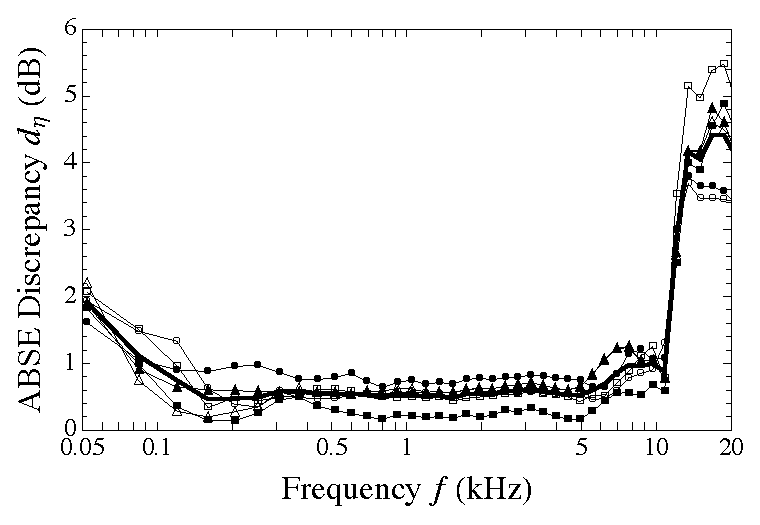
\includegraphics[width = 0.55\textwidth]{10_experimental_validation/figures/scharer2009_fullexp_F.eps}
  \caption[Experimental discrepancies in coloration spectra.]{
  Average discrepancies in ABSE spectra between simulations and measurements.
  Discrepancies are plotted for both the weighted average method (denoted by filled symbols) and the proposed method (empty symbols),
  as well as for each source: A ($\triangle$), B ($\square$), and C ($\bigcirc$).
  For each source and method combination, a thin black line connects the data points, while a thick black line indicates the average over all six curves.}
  \label{fig:10_Experimental_Validation:ABSE_Freq_Discrepancy}
\end{figure}

In \figref{fig:10_Experimental_Validation:ABSE_Freq_Discrepancy}, we plot, as a function of frequency, these average discrepancies in ABSE between the simulations and measurements for each navigation method and source position.
From this plot, we see that the simulations consistently match, within $\sim1$~dB, the physical measurements over a frequency range of approximately $150$~Hz to $10$~kHz.
The sharp increase in discrepancy at high frequencies can be explained by spatial aliasing,
a well-known effect which we do not model in our simulations (see \citet{Rafaely2005a}, for example).
The gradual increase in discrepancy at low frequencies, however, is explained by a combination of a) mismatches between the near-field compensation filters, b) non-anechoic conditions below $\sim425$~Hz, and c) low-frequency ambient noise in the measurements.

\begin{figure}[t]
\centering
  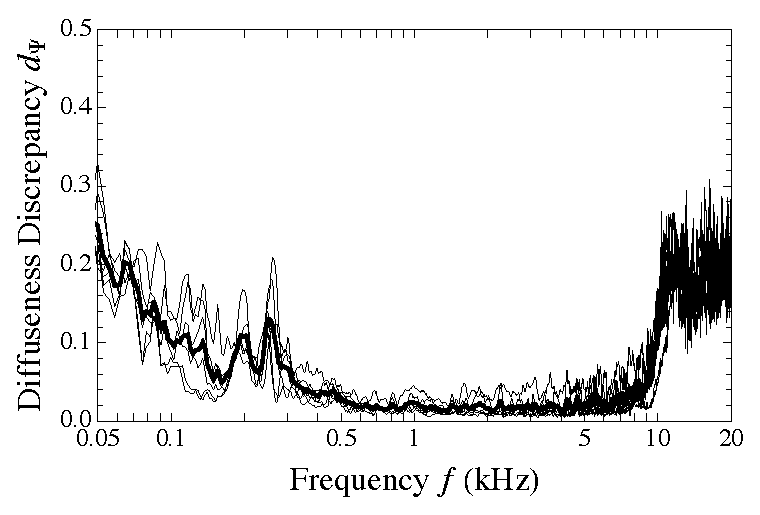
\includegraphics[width = 0.55\textwidth]{10_experimental_validation/figures/merimaa2005_fullexp_F.eps}
  \caption[Experimental discrepancies in diffuseness spectra.]{
  Average discrepancies in diffuseness spectra between simulations and measurements.
  Discrepancies are plotted for both the weighted average method and the proposed method,
  as well as for each source.
  For each source and method combination, a thin black line connects the data points, while a thick black line indicates the average over all six curves.}
  \label{fig:10_Experimental_Validation:Diffuseness_Freq_Discrepancy}
\end{figure}

In \figref{fig:10_Experimental_Validation:Diffuseness_Freq_Discrepancy}, we plot, as a function of frequency, similarly averaged discrepancies in diffuseness (as defined in \secref{sec:04_Auditory_Models:Diffuseness_Parameter}) between the simulations and measurements, given by $d_\Psi(f) = |\Psi(f) - \Psi'(f)|$, for each navigation method and source position.
From this plot, we again see that the simulations consistently match, within $\sim0.1$, the physical measurements over a frequency range of approximately $300$~Hz to $10$~kHz.
Again, spatial aliasing at high frequencies and the other effects mentioned above at low frequencies are evident.

\begin{figure}[t]
    	\centering
    	\begin{subfigure}[b]{0.49\textwidth}
		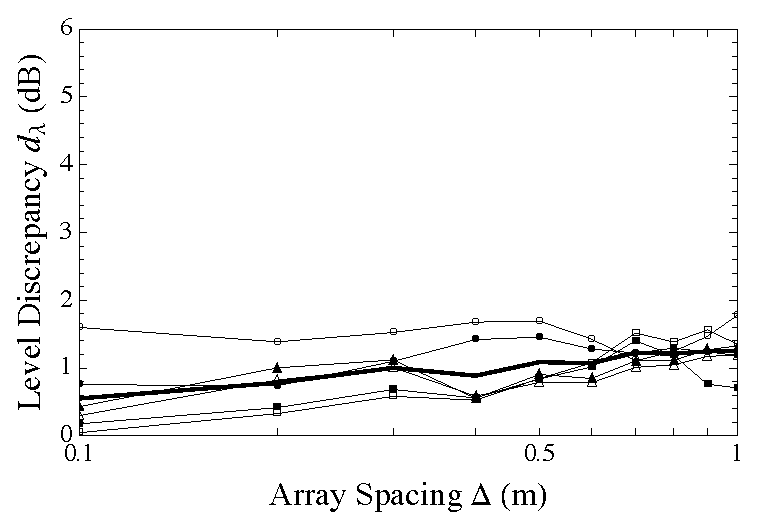
\includegraphics[width=\textwidth]{10_experimental_validation/figures/audibleEnergy_fullexp_D.eps}
		\caption{Level discrepancies}
		\label{fig:10_Experimental_Validation:MAE_Delta_Discrepancy}
    	\end{subfigure}
	\hfill
	\begin{subfigure}[b]{0.49\textwidth}
		\includegraphics[width=\textwidth]{10_experimental_validation/figures/scharer2009_fullexp_D.eps}
		\caption{ABSE discrepancies}
		\label{fig:10_Experimental_Validation:ABSE_Delta_Discrepancy}
    	\end{subfigure}
	
	\vspace{0.5cm}
	\begin{subfigure}[b]{0.49\textwidth}
		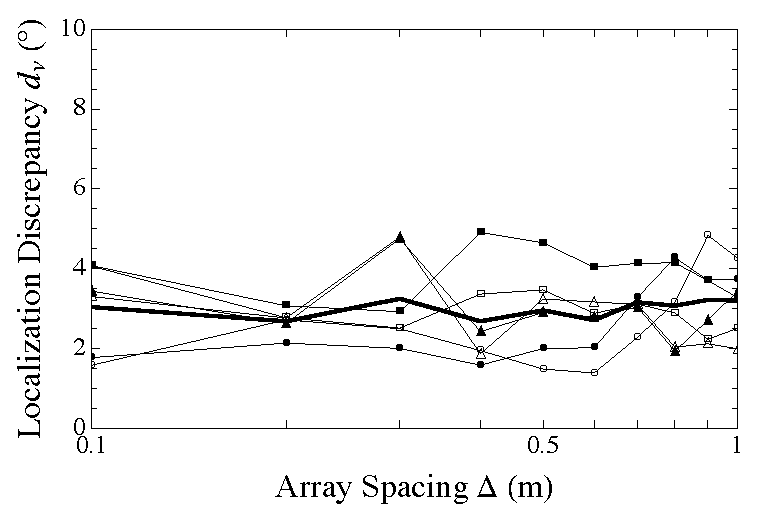
\includegraphics[width=\textwidth]{10_experimental_validation/figures/tylka2017_fullexp_D.eps}
		\caption{Localization discrepancies}
		\label{fig:10_Experimental_Validation:rPE_Delta_Discrepancy}
    	\end{subfigure}
	\hfill
	\begin{subfigure}[b]{0.49\textwidth}
		\includegraphics[width=\textwidth]{10_experimental_validation/figures/merimaa2005_fullexp_D.eps}
		\caption{Diffuseness discrepancies}
		\label{fig:10_Experimental_Validation:Diffuseness_Delta_Discrepancy}
    	\end{subfigure}
	
    	\caption[Experimental discrepancies for each microphone spacing.]{
	Discrepancies in level (top left panel), ABSE (top right), localization direction (bottom left), and diffuseness (bottom right), all plotted for each microphone spacing.
	The ABSE and diffuseness discrepancy spectra were first averaged over $[0,10]$~kHz.
  See \figref{fig:10_Experimental_Validation:ABSE_Freq_Discrepancy} for a description of the lines and symbols used.}
    	\label{fig:10_Experimental_Validation:Delta_Discrepancies}
\end{figure}

In \figref{fig:10_Experimental_Validation:MAE_Delta_Discrepancy}, we plot, now as a function of microphone spacing, the average discrepancies in level (as defined in \secref{sec:04_Auditory_Models:Audible_Energy}), given by $d_\lambda = |\lambda - \lambda'|$, where the average is taken over \textit{all} intermediate microphone positions for each microphone spacing.
From this plot, we see that the level discrepancies are consistently smaller than 2~dB, with a very slight and gradual increase with increasing microphone spacing.

In \figref{fig:10_Experimental_Validation:ABSE_Delta_Discrepancy}, we plot the average discrepancies in ABSE, where two averages are taken: first over all frequencies $f_c \in [0,10]$~kHz and subsequently over all strictly interior intermediate microphone positions.
From this plot we see that the discrepancy between simulation and measurement is consistently smaller than $1$~dB, again with a very slight and gradual increase with increasing microphone spacing.

Given the simulated and measured localization directions (from the localization model described in \secref{sec:05_Proposed_Models:Localization_Model}), we next compute the discrepancy, $d_\nu = \cos^{-1} \left( \hat{\nu} \cdot \hat{\nu}' \right)$, for each navigation method, source position, microphone spacing, and intermediate microphone position.
In \figref{fig:10_Experimental_Validation:rPE_Delta_Discrepancy}, we plot, as a function of microphone spacing, averages of these discrepancies over all strictly interior intermediate microphone positions.
From this plot we see that the discrepancy between simulation and measurement is consistently smaller than $5^\circ$, with an average value of approximately $3.5^\circ$, and does not vary significantly with microphone spacing.

Finally, in \figref{fig:10_Experimental_Validation:Diffuseness_Delta_Discrepancy}, we plot the average discrepancies in diffuseness, where again two averages are taken: first over all frequencies $f \in [0,10]$~kHz and subsequently over all strictly interior intermediate microphone positions.
From this plot we see that the discrepancy between simulation and measurement is consistently smaller than $0.1$ and does not vary significantly with microphone spacing.

Taken together, \figrefthru{fig:10_Experimental_Validation:ABSE_Freq_Discrepancy}{fig:10_Experimental_Validation:Delta_Discrepancies} further suggest that the discrepancies between simulations and measurements do not depend significantly on navigational method or source position.

\section{Conclusions}\label{sec:10_Experimental_Validation:Conclusions}
In order to validate our numerical simulations, we conducted a set of acoustical measurements, as described in \secref{sec:10_Experimental_Validation:Experiments}, taken over a subset of the simulated conditions presented in \chapref{chap:08_Proposed_Method}.
Results of these measurements are in good agreement with those of the simulations, indicating that our simulations are indeed representative of reality.
In particular, spectral error discrepancies are consistently smaller than $1$~dB and diffuseness discrepancies are consistently smaller than $0.1$ across all frequencies within approximately $300$~Hz to $10$~kHz.%
\footnote{The significant discrepancies observed at high frequencies can be explained by spatial aliasing, an effect which we do not currently account for in our simulations, but could potentially be incorporated in the future with a simple model based on the geometrical arrangement of capsules on the spherical microphone array used in the measurements.}
Additionally, level discrepancies are consistently within $2$~dB and localization direction discrepancies are consistently within $5^\circ$ ($3.5^\circ$ on average) across all microphone spacings.
A more comprehensive validation of our simulation framework could consider alternative navigational methods and span wider ranges of microphone spacings and source positions.
However, as expected, the present results suggest that the observed discrepancies (and therefore the fidelity of the simulations) do not depend significantly on the navigational method, microphone spacing, or source position.

\section*{Acknowledgements}
The ambisonics room impulse responses were recorded using the Eigenmike by mh Acoustics \citep{EigenmikeURL}.
This work was originally submitted by \citet[section 6]{TylkaChoueiri2019b} to \textit{The Journal of the Audio Engineering Society}.